% -----------
% Copyright 2013-2015, Andrew Lindesay
% Distributed under the terms of the MIT License.
% -----------

\section{Data Model}

\begin{figure}
\centering
\vspace{.2in}
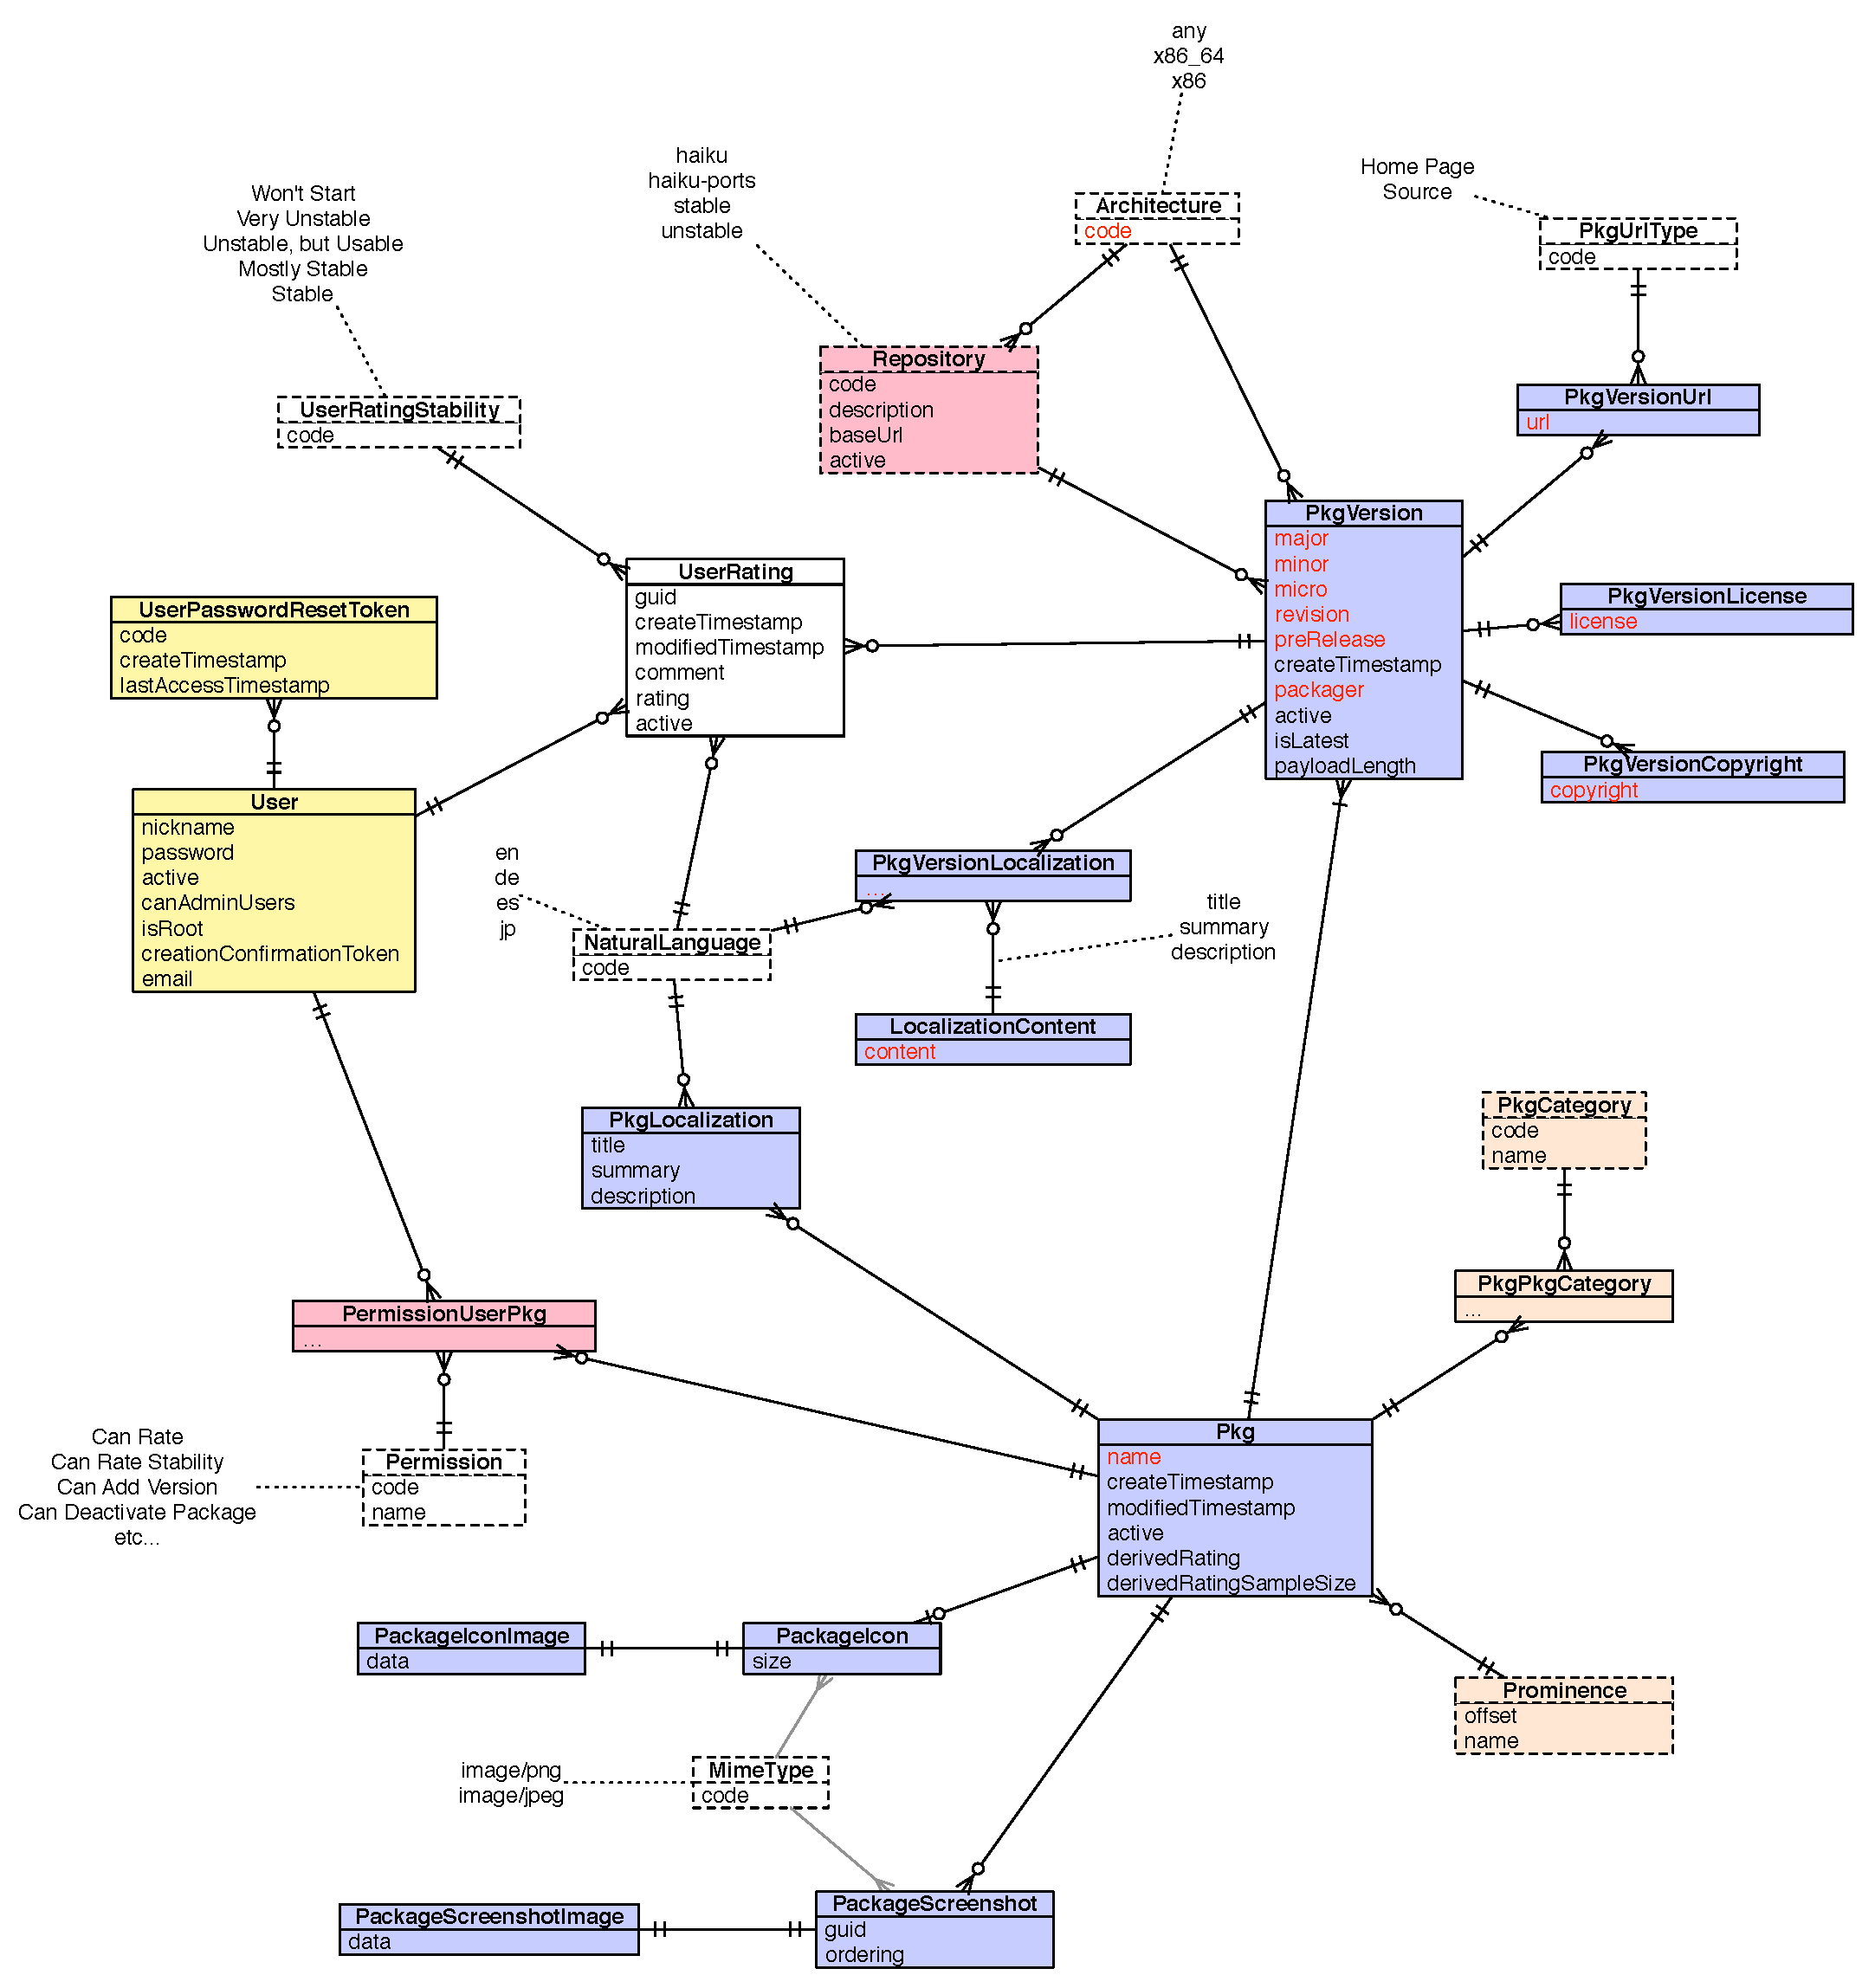
\includegraphics[width=6.5in]{img-datamodel.pdf}
\caption{Persisted data model for the Haiku Depot Server application.}
\label{\thefigure}
\end{figure}

Figure {\thefigure} shows the persisted data model for the application server.

\subsection{Unique Identifiers}

In general, an artifical attribute used to identify instances has a name of ``code''.  In some cases, existing nomenclature is already in place and another attribute name has been chosen.  An example of this is the ``Pkg'' entity which is uniquely identified by its attribute ``name''.

